%%%%%%%%%%%%%%%%%%%%%%%%%%%%%%%%%%%%%%%%%
% University/School Laboratory Report
% LaTeX Template
% Version 2.0 (4/12/12)
%
% This template has been downloaded from:
% http://www.latextemplates.com
%
% License:
% CC BY-NC-SA 3.0 (http://creativecommons.org/licenses/by-nc-sa/3.0/)
%
% Original header:
%
% This is a LaTeX version of the sample laboratory report
% from Virginia Tech's copyrighted 08-09 CHEM 1045/1046 lab manual.
% Reproduction of this one appendix section for academic purposes
% should fall under fair use.
%
%%%%%%%%%%%%%%%%%%%%%%%%%%%%%%%%%%%%%%%%%

\documentclass{article}

\usepackage{graphicx} % Allows the inclusion of images

\title{ELEC 302-81\\ Lab 1\\ Power in AC Circuits} % Title

% \author{John \textsc{Smith}} % Author name

\date{\today} % Specify a date for the report

\begin{document}

\maketitle

\begin{center}
  \begin{tabular}{l r}
    Date Performed: & January 14, 2013 \\
    Partners: & John Doe \\
              & Charles Pittman \\
    Instructor: & Dr. Weatherford
  \end{tabular}
\end{center}

\pagebreak

\setlength\parindent{0pt} % Removes all indentation from paragraphs

% Make numbering in the enumerate environment by letter rather than number
% (e.g. section 6)
\renewcommand{\labelenumi}{\alph{enumi}.} 

\section{Introduction}

\section{Procedure}

\section{Results}

\section{Conclusion}

\section{Calculated Data}
\begin{table}[h]
  \begin{center}
    \begin{tabular}{cccccccccc}
      R      & L & C      & I$_1$ & E$_1$ & P & \theta & S & Q & p.f. \\
      \Omega & H & \mu{F} & A & V & W & \deg & VA & VAR & \\
      \hline
      1200 & 0.8 & --- & 0.210 & 60 & 4.56 &  68.77 & 12.58 & 11.73 & 0.36 \\
      1200 & 0.8 & 2.2 & 0.164 & 60 & 4.56 &  62.48 &  9.86 &  8.75 & 0.46 \\
      1200 & 0.8 & 4.4 & 0.122 & 60 & 4.56 &  51.65 &  7.34 &  5.76 & 0.62 \\
      1200 & 0.8 & 8.8 & 0.076 & 60 & 4.56 &  -2.67 &  4.56 & -0.21 & 1.00 \\
      1200 & 1.6 & --- & 0.114 & 60 & 3.39 &  60.27 &  6.84 &  5.94 & 0.50 \\
      1200 & 1.6 & 2.2 & 0.075 & 60 & 3.39 &  41.06 &  4.50 &  2.96 & 0.75 \\
      1200 & 1.6 & 4.4 & 0.057 & 60 & 3.39 &  -0.50 &  3.39 & -0.03 & 1.00 \\
      1200 & 1.6 & 8.8 & 0.115 & 60 & 3.39 & -60.51 &  6.89 & -6.00 & 0.49
    \end{tabular}
    \caption{Calculated Data}
    \label{calc_dat}
  \end{center}
\end{table}

\section{Experimental Data}
\begin{table}[h]
  \begin{center}
    \begin{tabular}{cccccccccc}
      R      & L & C      & I$_1$ & E$_1$ & P & \theta & S & Q & p.f. \\
      \Omega & H & \mu{F} & A & V & W & \deg & VA & VAR & \\
      \hline
      1200 & 0.8 & --- & 0.206 & 60.9 & 4.53 &  68.0 & 12.58 & 11.73 & 0.36 \\
      1200 & 0.8 & 2.2 & 0.158 & 60.9 & 4.56 &  60.9 &  9.86 &  8.75 & 0.46 \\
      1200 & 0.8 & 4.4 & 0.117 & 60.9 & 4.59 &  49.0 &  7.34 &  5.76 & 0.62 \\
      1200 & 0.8 & 8.8 & 0.081 & 61.0 & 4.65 &  -4.4 &  4.56 & -0.21 & 1.00 \\
      1200 & 1.6 & --- & 0.116 & 61.0 & 3.94 &  55.4 &  6.84 &  5.94 & 0.50 \\
      1200 & 1.6 & 2.2 & 0.079 & 61.0 & 3.96 &  32.8 &  4.50 &  2.96 & 0.75 \\
      1200 & 1.6 & 4.4 & 0.067 & 61.0 & 3.99 &  -6.6 &  3.39 & -0.03 & 1.00 \\
      1200 & 1.6 & 8.8 & 0.124 & 61.2 & 4.05 & -57.4 &  6.89 & -6.00 & 0.49 \\
    \end{tabular}
    \caption{Experimental Data}
    \label{meas_dat}
  \end{center}
\end{table}

\begin{figure}
\begin{center}
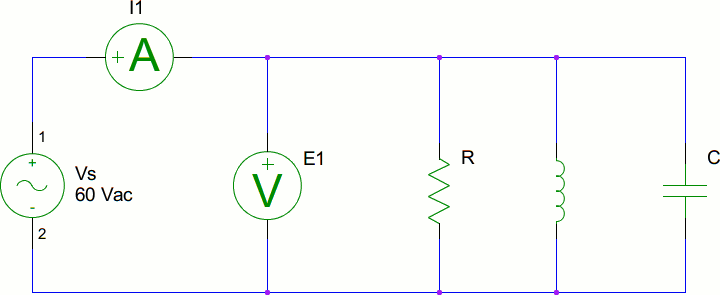
\includegraphics[width=\textwidth]{test_circuit} % Include the image placeholder.png
\caption{Parallel RLC Circuit Configuration}
\end{center}
\end{figure}

\end{document}
